% Tento soubor nahraďte vlastním souborem s přílohami (nadpisy níže jsou pouze pro příklad)

% Pro kompilaci po částech (viz projekt.tex), nutno odkomentovat a upravit
%\documentclass[../projekt.tex]{subfiles}
%\begin{document}

% Umístění obsahu paměťového média do příloh je vhodné konzultovat s vedoucím
%\chapter{Obsah přiloženého paměťového média}

\chapter{Příklady zdrojových kódů v~jazyce Koubp a~jejich AST reprezentace}

\section{Příkaz if-elseif}
\begin{lstlisting}[language=Koubp]
    if (vyraz)
        prikaz();
    elseif(vyraz)
        prikaz();
\end{lstlisting}
\begin{figure}[ht]
    \centering
    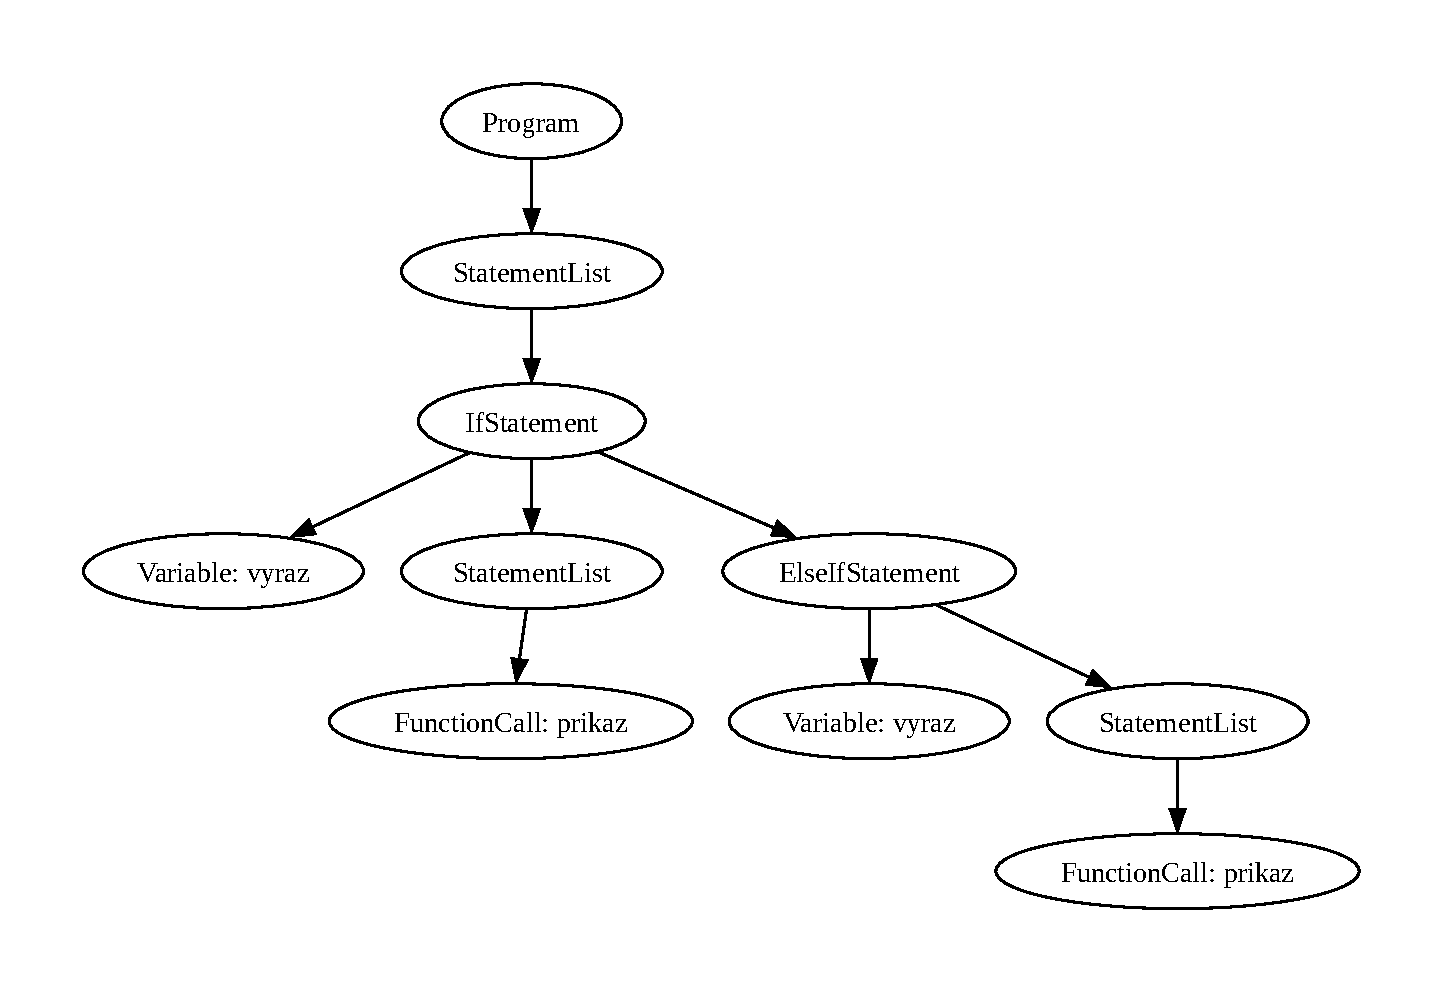
\includegraphics[width=\textwidth]{obrazky-figures/ast_if_elseif.pdf}
    \caption{Programem vygenerovaný AST pro konstrukci \texttt{if-elseif}}
    \label{fig_ast_elseif}
\end{figure}

\section{Příkaz if-else if}
\begin{lstlisting}[language=Koubp]
    if (vyraz)
        prikaz();
    else if(vyraz)
        prikaz();
\end{lstlisting}
\begin{figure}[ht]
    \centering
    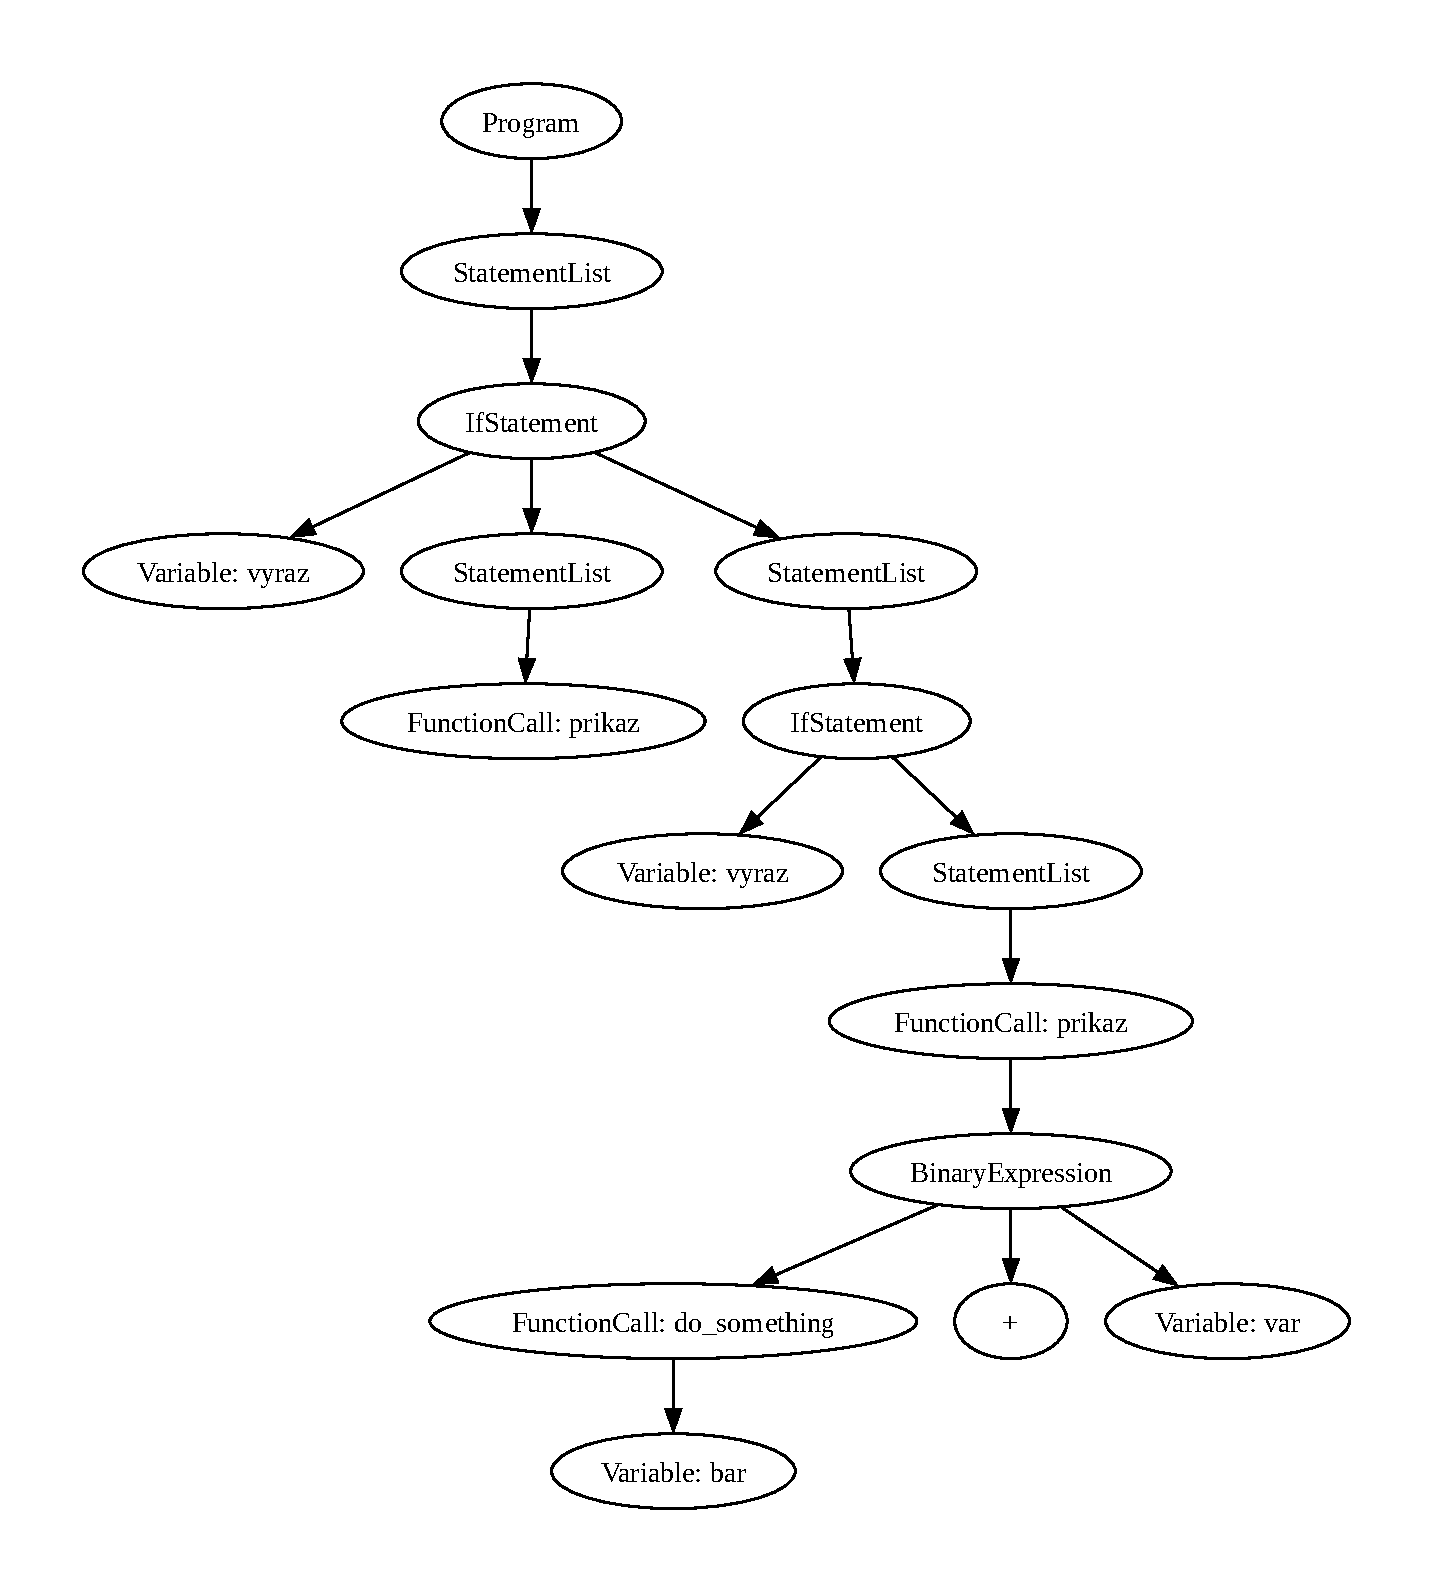
\includegraphics[width=\textwidth]{obrazky-figures/ast_if_else_if.pdf}
    \caption{Programem vygenerovaný AST pro konstrukci \texttt{if-else if}}
    \label{fig_ast_else_if}
\end{figure}

\newpage

\section{For cyklus}

\begin{lstlisting}[language=Koubp]
	for (int i = 0; i < 2; i = i + 1) {}
\end{lstlisting}

\vspace{11em}

\begin{figure}[h]
	\centering
	\begin{sideways}
		\begin{minipage}{\linewidth}
			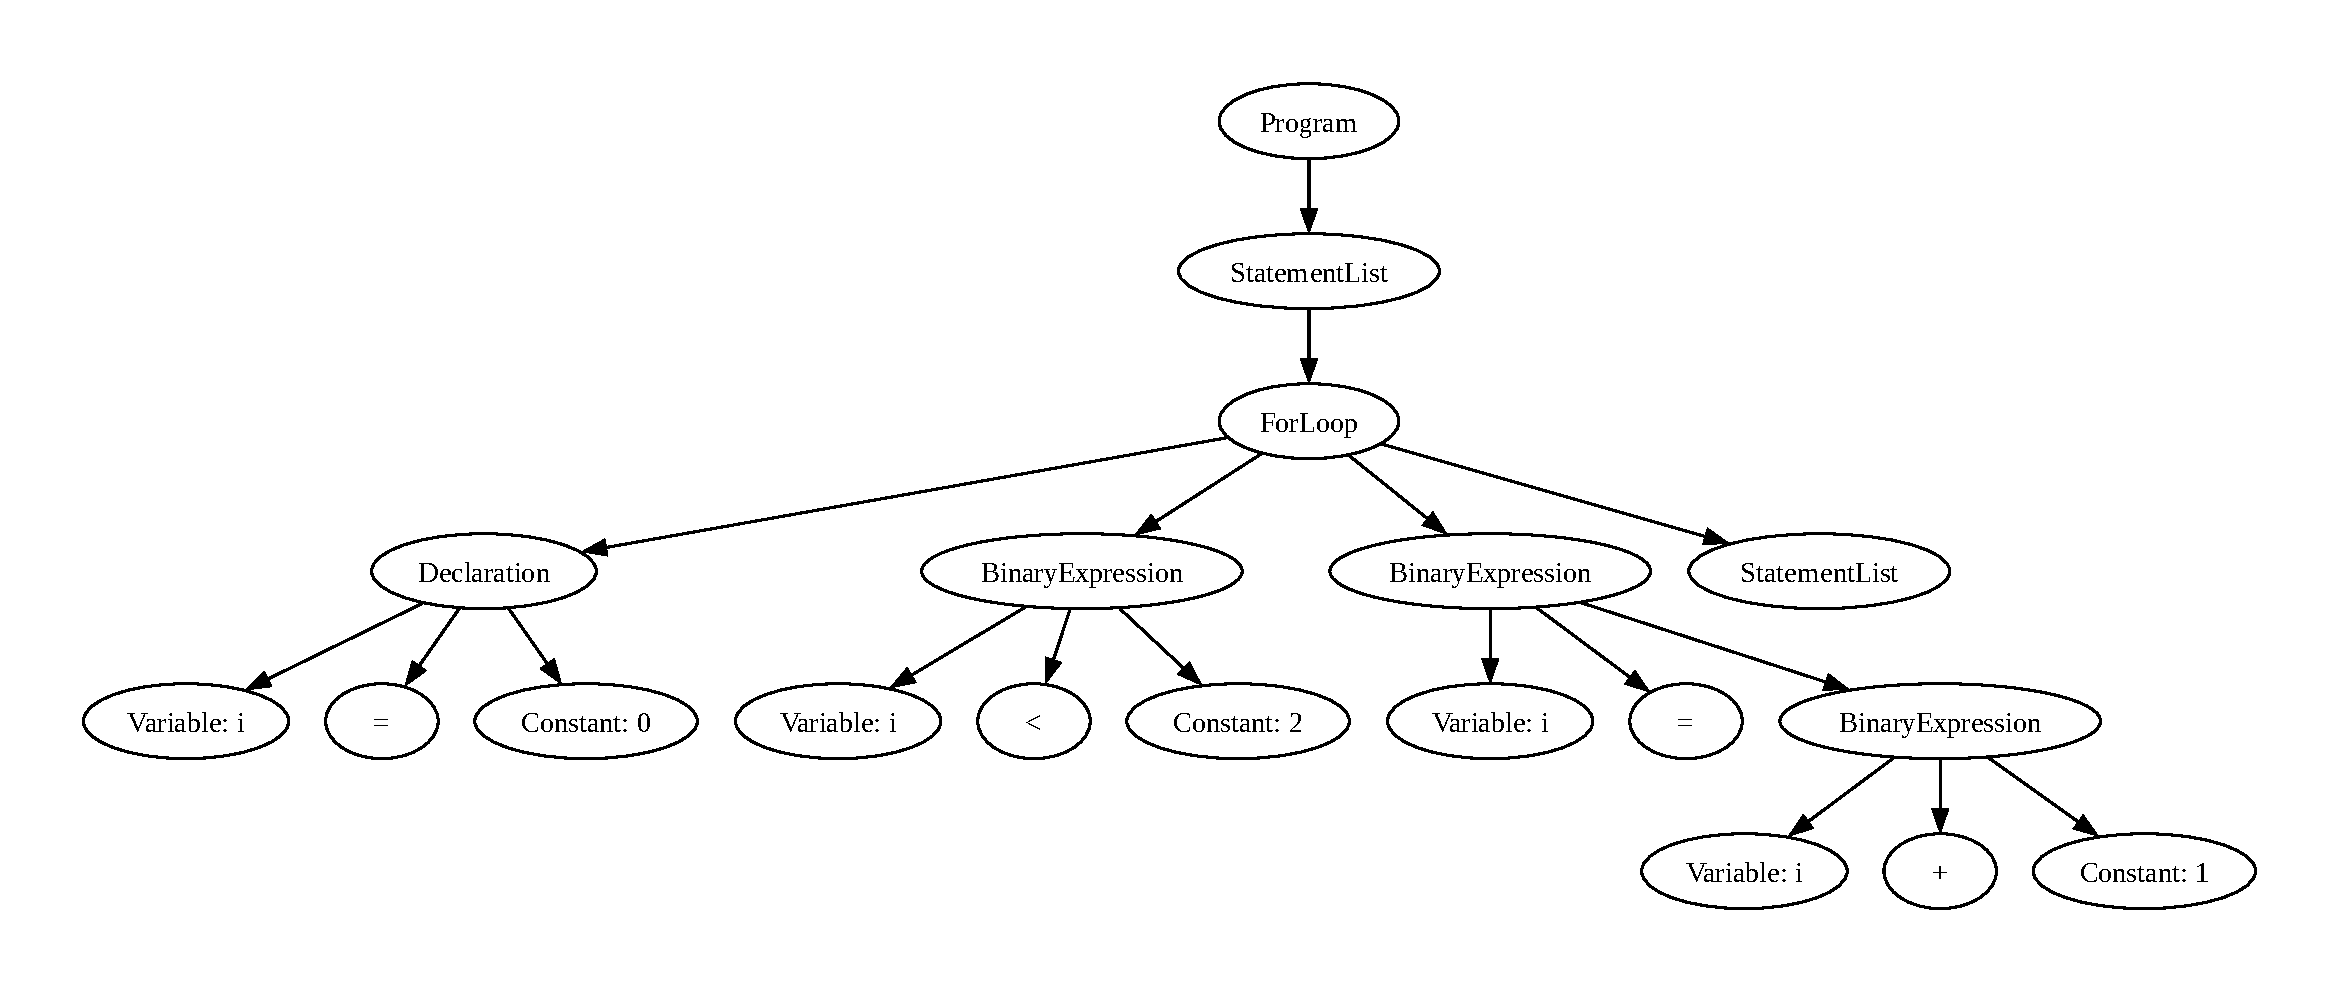
\includegraphics[width=1.3\textwidth, keepaspectratio]{obrazky-figures/tree_for.pdf}
			\vspace{1em}
		\end{minipage}
	\end{sideways}
	\caption{Programem vygenerovaný AST pro cyklus \texttt{for}. Pro lepší čitelnost obrázek otočen o~90°.}
	\label{fig_ast_cyklus_for}
\end{figure}



\newpage
\section{Deklarace a přiřazení}

\begin{lstlisting}[language=Koubp]
    float input = do_something(var, f(1) + 2) + 20.0*d;
\end{lstlisting}
\begin{figure}[h]
    \centering
    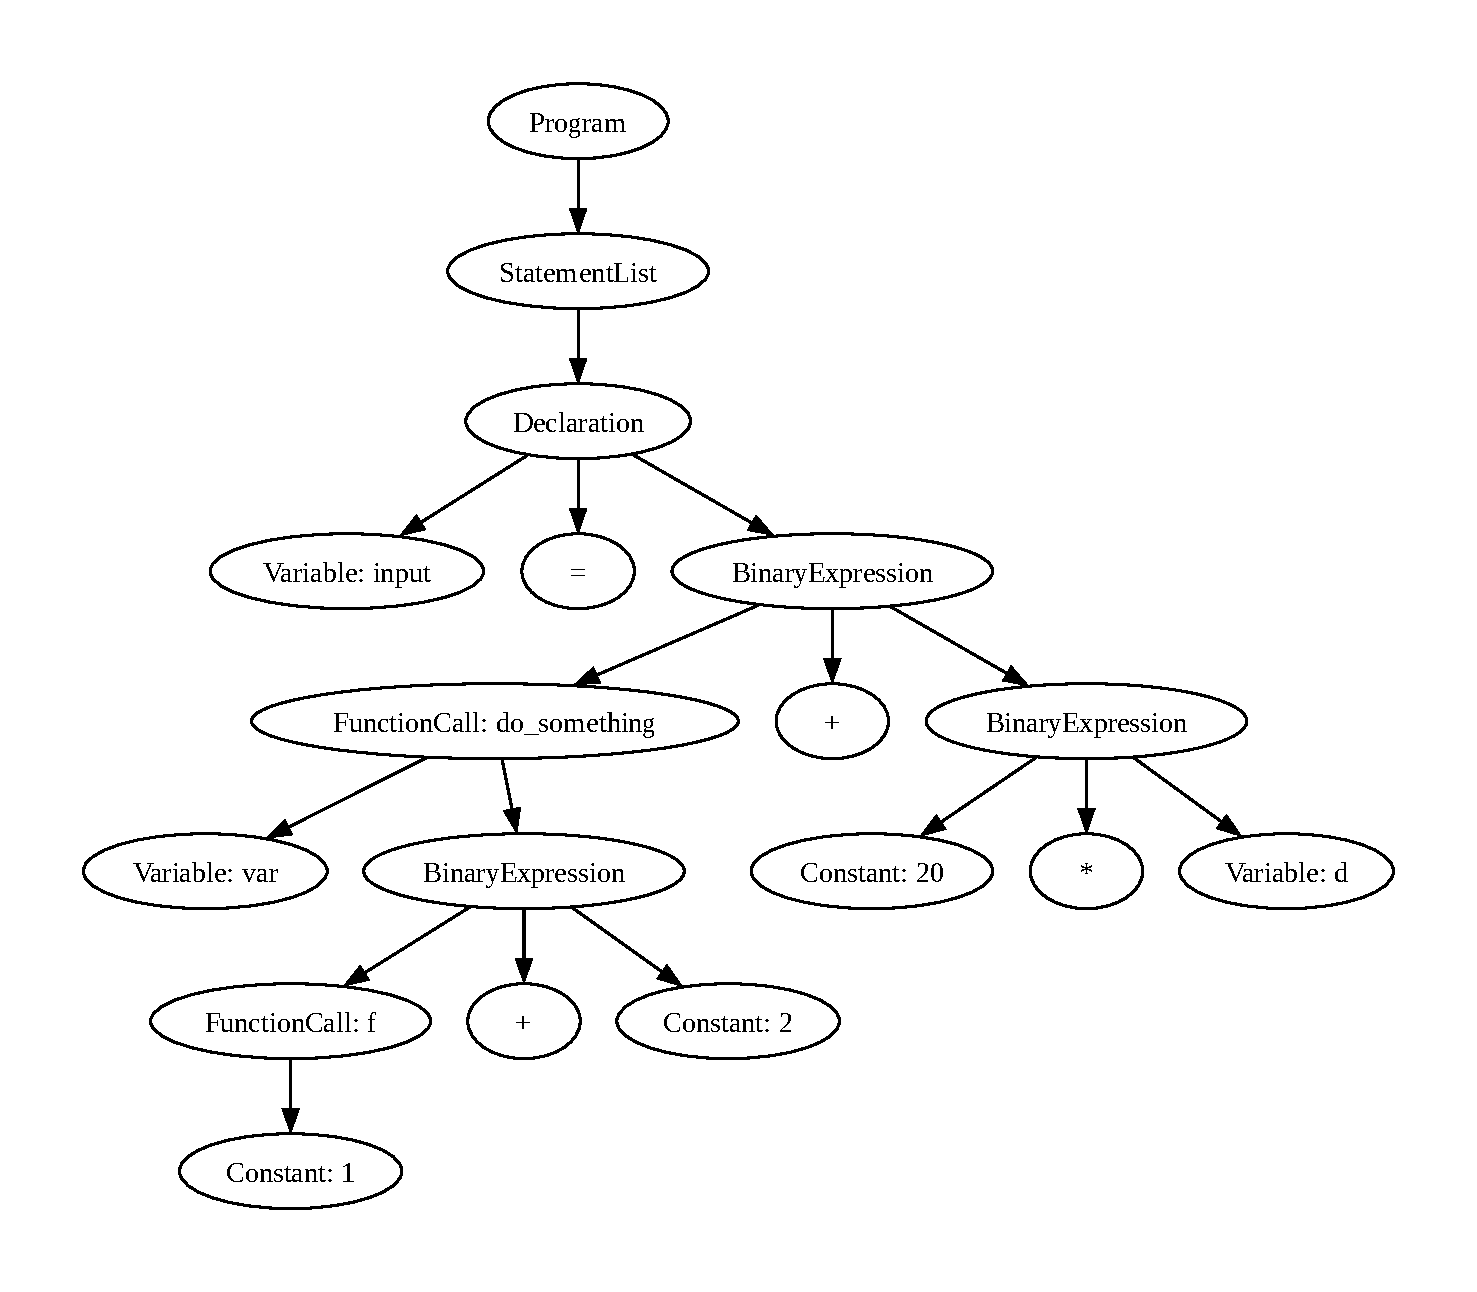
\includegraphics[width=\textwidth]{obrazky-figures/tree_deklarace.pdf}
    \caption{Programem vygenerovaný AST pro deklaraci s~přiřazením.}
    \label{fig_ast_declaration}
\end{figure}


\chapter{Vztahy tříd provádějící syn\-tak\-tic\-kou analýzu}\label{kap_priloha_b}

Třídní diagram na obrázku \ref{fig_parsers_class_diagram} obsahuje pouze třídy, které se starají o~algoritmus syntaktické analýzy, respektive simulaci zásobníkového automatu.
Další pomocné třídy, jako například LL tabulka nebo precedenční tabulka, nejsou do grafu přidány kvůli přehlednosti vzhledem k~velikosti diagramu.
\begin{figure}[ht]
    \centering
    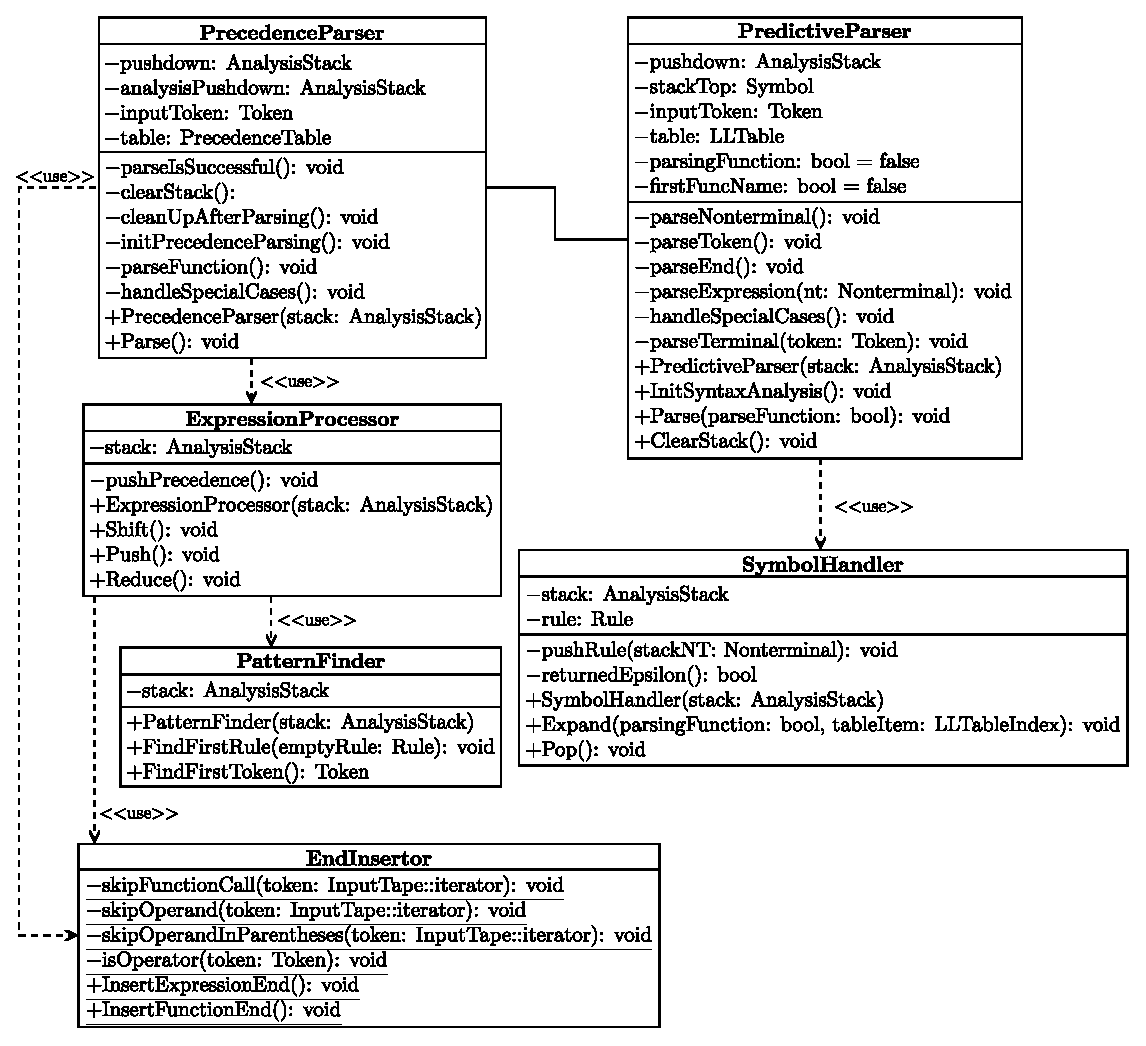
\includegraphics[width=0.92\textwidth]{obrazky-figures/parsers_class_diagram.eps}
    \caption{Vztahy mezi třídami, které spolupracují na syntaktické analýze.}
    \label{fig_parsers_class_diagram}
\end{figure}

\chapter{Třídní hierarchie uzlů AST} \label{kap_priloha_c}
Pro větší přehlednost je hierarchie rozdělena do tří obrázků. Tyto diagramy jsou úmyslně zjednodušené, zaměřují se pouze na vzájemnou dědičnost mezi třídami; opomíjí kompoziční vztahy a~další detaily, jako například jiné a~ne tak podstatné třídy, použité enumerátory a~podobně. Jejich hlavním účelem je ilustrovat strukturu hierarchie uzlů AST.

První obrázek (Obrázek \ref{fig_hierarchie_astnode}) ukazuje třídu \texttt{ASTNode} a~třídy, které z~ní přímo dědí.
\begin{figure}[h]
	\centering
	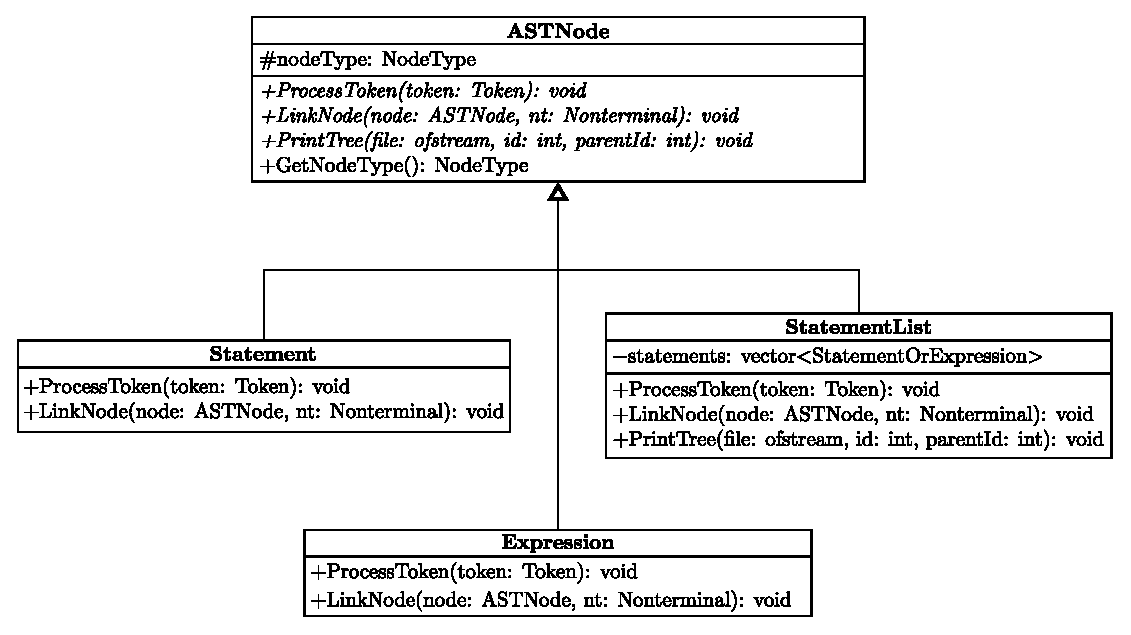
\includegraphics[width=\textwidth]{obrazky-figures/ast_node_hierarchy.eps}
	\caption{Diagram tříd zobrazující třídu \texttt{ASTNode} a~její přímé potomky.}
	\label{fig_hierarchie_astnode}
\end{figure}
\newpage

Druhý obrázek (Obrázek \ref{fig_hierarchie_expression}) prezentuje hierarchii tříd, které reprezentují různé typy výrazů v~AST. 
\begin{figure}[h]
	\centering
	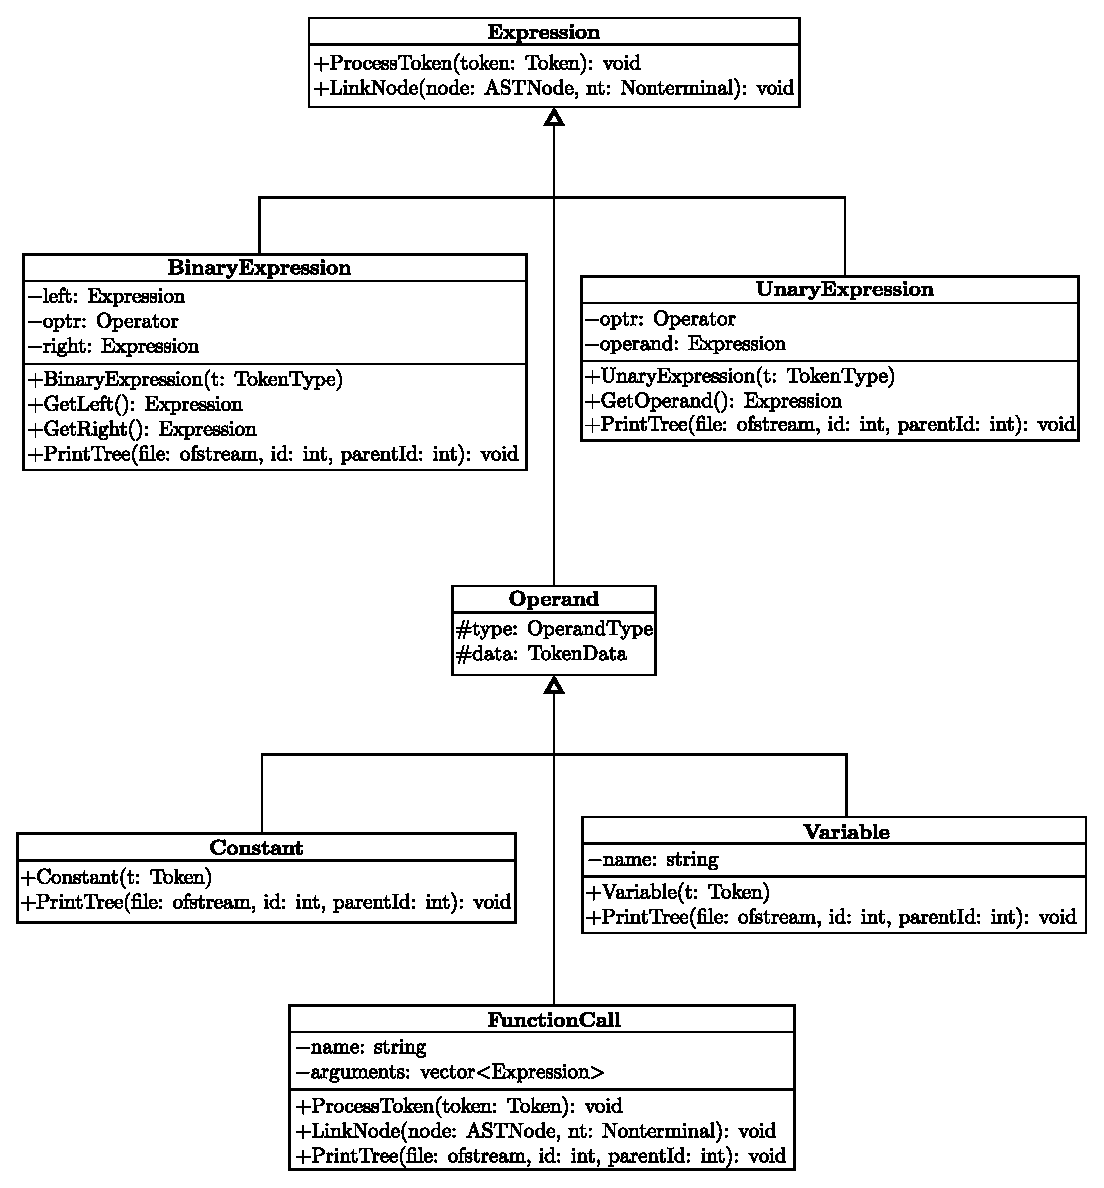
\includegraphics[width=\textwidth]{obrazky-figures/expression_hierarchy.eps}
	\caption{Třídní hierarchie AST pro všechny typy výrazů.}
	\label{fig_hierarchie_expression}
\end{figure}
\newpage

Třetí diagram na Obrázku \ref{fig_hierarchie_statement} zobrazuje různé druhy příkazů ve zdrojovém kódu pomocí tříd. Podobně jako u~předchozích diagramů, tento diagram se soustředí na hierarchii těchto tříd a~vynechává zbytečné detaily.
\begin{figure}[h!]
		\centering
		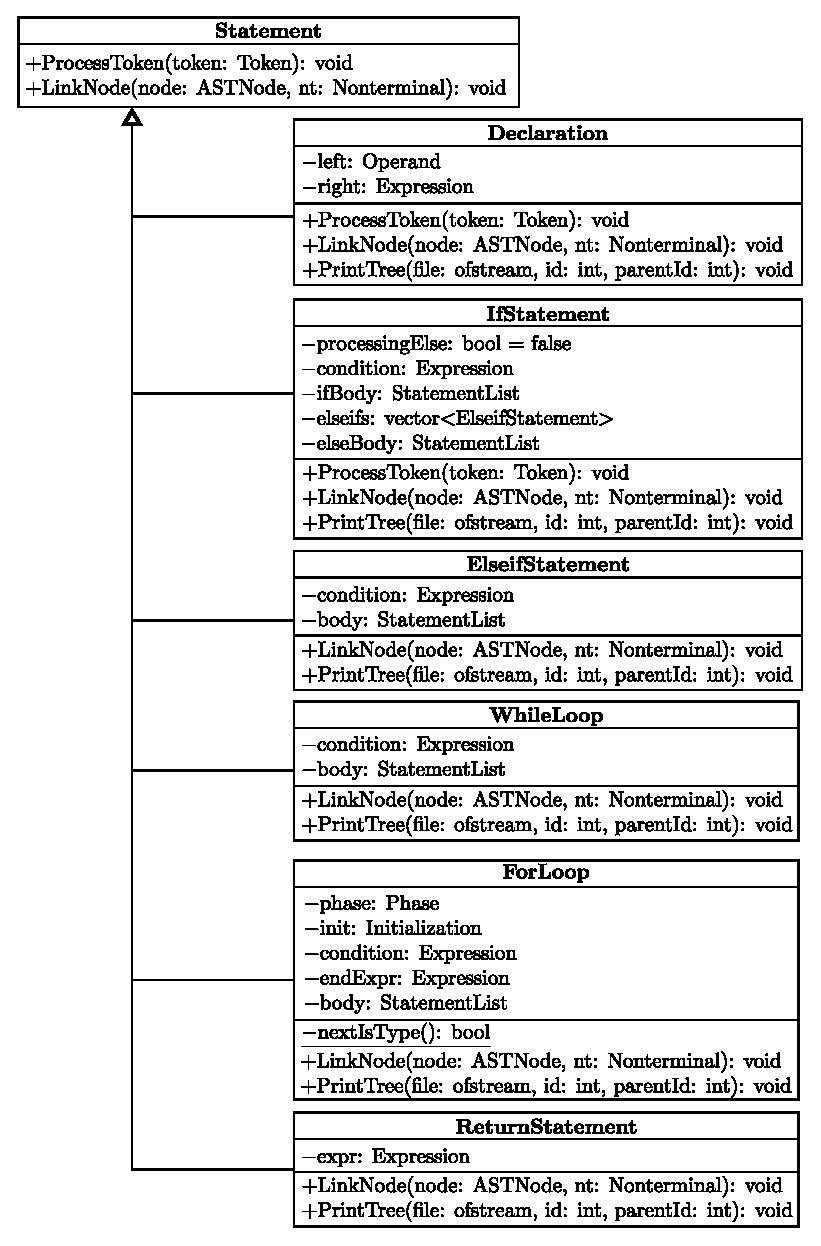
\includegraphics[height=0.88\textheight]{obrazky-figures/statement_hierarchy.eps}
		\caption{Třídní diagram s~třídami uzlů AST, které reprezentují příkazy.}
		\label{fig_hierarchie_statement}
\end{figure}
%\chapter{Plakát}



% Pro kompilaci po částech (viz projekt.tex) nutno odkomentovat
%\end{document}
